\documentclass{article}

\usepackage{amsmath}
\usepackage{amssymb}
\usepackage{geometry}
\usepackage{graphicx}
\usepackage{minted}
\usepackage[shortlabels]{enumitem}
\usepackage[style=ieee, url=false]{biblatex}
\addbibresource{bibliography/jetpump.bib}
\usepackage{float}
\usepackage{commath}

% Make header with name and date etc.
\usepackage{fancyhdr}
\lhead{Kaelin Ellis\\Math F661: Optimization}
\rhead{\today\\Project Submission}
\pagestyle{fancy}

\usepackage[utf8]{inputenc}
\setlength{\parindent}{0pt} % Don't indent new paragraphs
\setlength{\headheight}{24pt} 

% Import titlesec package for customizing section titles
\usepackage{titlesec}

% Redefine \section to be non-bold and without numbers
\titleformat{\section}
  {\bfseries\large} % Bold font (\bfseries) and large size
  {} % No numbering
  {0pt} % No extra spacing
  {} % No special formatting before section title

\begin{document}

\begin{center}
    \Large Title: Optimizing Power Fluid in Jet Pumps \par
\end{center}

\section{Introduction}

Oil wells on jet pumps have to share a common resource called power fluid to assist with lifting the well to surface. If the power fluid is unlimited, then an unconstrained optimization problem exists and each well can be lifted with the max power fluid required. In mature fields with many wells, this is not the condition, and the wells are required to share a finite resource of power fluid. As such an optimization scheme needs to be developed to appropriately divide the power fluid to maximize oil production. A network overview of four wells sharing power fluid from a common kinetic pump is shown in figure \ref{fig:jetpump_network}.

\begin{figure}[H]
    \centering
    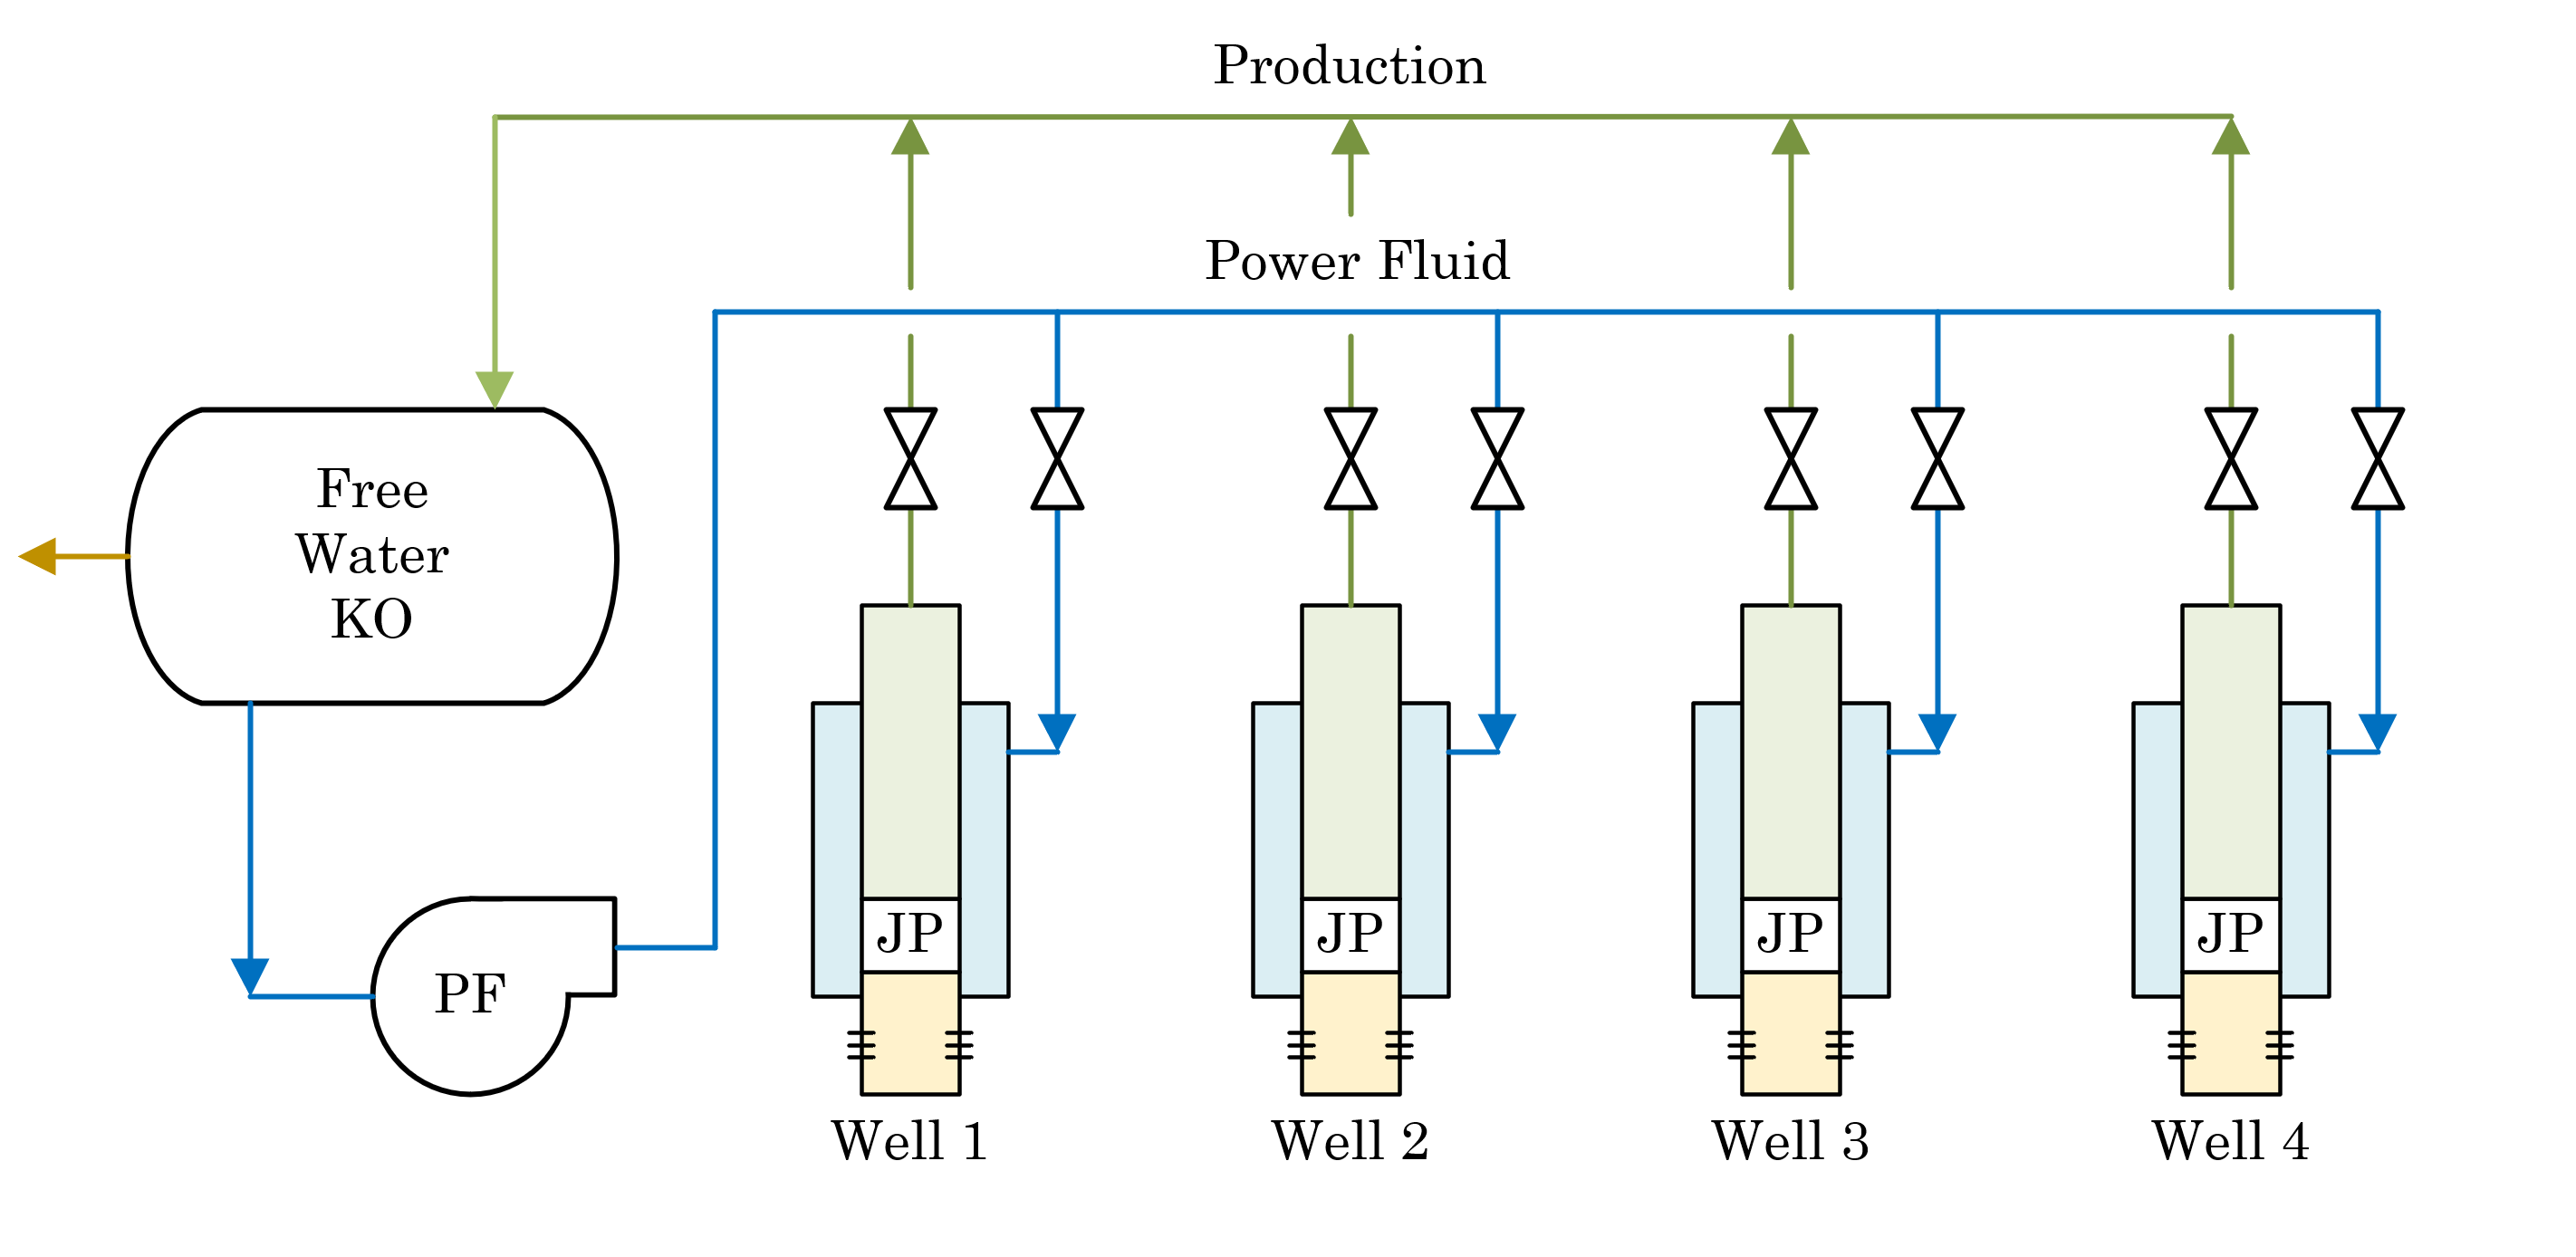
\includegraphics[width=1\linewidth]{figures/network_diagram.PNG}
    \caption{Network Diagram of Four Wells}
    \label{fig:jetpump_network}
\end{figure}

\section{Mathematical Model}

The oil production from a well on jet pump is represented with the equation below. Where $q_{o}$ is the oil produced and $q_{p}$ is the power fluid volume required.

\begin{equation*}
    q_{oi} = c_{1i} - c_{2i} \exp{(-q_{pi} c_{3i})}
\end{equation*}

The coefficients $c_{1}$, $c_{2}$ and $c_{3}$ for each well are found in a separate numerical scheme and are dependent on the specific wells water cut, formation gas oil ratio and specific subsurface geometry. The optimization objective function and constraints are as follows:

\begin{equation*}
\begin{aligned}
    \text{maximize } & f(x) = \sum_{i=1}^{n} q_{o\:i} \\
    \text{subject to } & \sum_{i=1}^{n} q_{p\:i} \leq Q_{\text{p}}^{\text{tot}} \\
    & q_{p\:i} \geq 0 \\
\end{aligned}
\end{equation*}

The index $i$ represents a specific unique oil well that is on the network. The vector $x$ represents the individual power fluid to each well $x = (q_{p\:1}, q_{p\:2}, ..., q_{p\:n})^{T}$.

\section{Reduced Newton's Method with Active Set Constraints}

A reduced Newton method is used for finding direction, while an active set is used to handle the constraints. The active set method is solving a problem of the form.

\begin{equation*}
\begin{aligned}
    \text{minimize  } & f(x) \\
    \text{subject to  } & \hat{A}x = \hat{b}
\end{aligned}
\end{equation*}

$\hat{A}$ and $\hat{b}$ are the active inequality $\hat{\mathcal{I}}$ and equality $\mathcal{E}$ constraints. The null space of the active constraints is $\hat{Z}$. The null space is part of the reduced gradient $\nabla \phi (v)$ and reduced Hessian $\nabla^{2} \phi (v)$.

$$\nabla \phi (v) = \hat{Z}^{T}\nabla f(x) \qquad \nabla^{2} \phi (v) = \hat{Z}^{T}\nabla^2 f(x) \hat{Z}$$

The reduced gradient and Hessian are used in the \textit{reduced Newton direction} equation shown below.

$$p = \hat{Z}v = -\hat{Z}(\underbrace{\hat{Z}^{T}\nabla^2 f(x_k)\hat{Z}}_{\nabla^{2}\phi(v)})^{-1}\underbrace{\hat{Z}^{T}\nabla f(x_{k}}_{\nabla \phi(v)})$$

While moving around, backtracking line search is used to guarantee descent of the objective function.

$$f(x_{k} + \alpha p) \leq f(x_{k}) + \mu \alpha p^T \nabla f(x_k)$$

The ratio test ensures no movement exceeds inactive constraints. 

\begin{equation*}
        \tau = \min \left\{ \dfrac{a_i^T \bar{x} - b_{i}}{-a_i^T p} : a_i^T p < 0, i \notin \hat{\mathcal{I}}, \mathcal{E} \right \}
\end{equation*}

Lagrange multiples are calculated to ensure the function can't be further reduced if an active constraint is made inactive. Depending on the results of the ratio test and Lagrange multiples, the active set  $\hat{A}$, $\hat{A}$ and $\hat{Z}$ are constantly updated to ensure feasibility. More detail on this can be found in chapters 15.2, 15.3 and 15.4 of the referenced textbook \cite{optm_griva}.

\section{Specific Equations}

The following section will show how our specific problem is transformed so it can be solved by the reduced Newton method with active set constraints. Since the problem is originally a maximization problem, the objective function needs to be multiplied by -1 to turn it into a minimization problem.

\begin{equation*}
\begin{aligned}
    \text{minimize } & f(x) = \sum_{i=1}^{n} - c_{1i} + c_{2i} \exp{(-q_{pi} c_{3i})} \\
    \text{subject to } & \sum_{i=1}^{n} q_{p\:i} \leq Q_{\text{p}}^{\text{tot}} \\
    & q_{p\:i} \geq 0 \\
\end{aligned}
\end{equation*}

The gradient of the objective function is the first derivative of each well with respect to its own power fluid.

\begin{equation*}
    \nabla f(x) = 
    \begin{pmatrix}
    - c_{21} c_{31} \exp{(-q_{p1} c_{31})} \\[6pt]
    ... \\[6pt]
    - c_{2n} c_{3n} \exp{(-q_{pn} c_{3n})} 
    \end{pmatrix}
\end{equation*}

Since each wells performance is only dependent on its own power fluid usage, the Hessian is a simple diagonal matrix.

\begin{equation*}
    \nabla^{2} f(x) = 
    \begin{pmatrix}
    c_{21} c_{31}^{2} \exp{(-q_{p1} c_{31})} & 0 & 0 \\[6pt]
    0 & ... & 0 \\[6pt]
    0 & 0 & c_{2n} c_{3n}^{2} \exp{(-q_{pn} c_{3n})} 
    \end{pmatrix}
\end{equation*}

The top $n$ rows of the constraint matrix $A$ and vector $b$ represent the individual wells. The bottom $n+1$ row represents the total power fluid limitation. The bottom row is multiplied by negative one to ensure adherence to $Ax \geq b$.

\begin{equation*}
    A = 
    \begin{pmatrix}
    1 & 0 & 0 \\[4pt]
    0 & ... & 0\\[4pt]
    0 & 0 & 1 \\[4pt]
    -1 & -1 & -1
    \end{pmatrix} \quad
    x_{k} = 
    \begin{pmatrix}
    q_{p1} \\[4pt]
    ... \\[4pt]
    q_{pn} \\
    \end{pmatrix} \quad
    b = 
    \begin{pmatrix}
    0 \\[4pt]
    ... \\[4pt]
    0 \\[4pt]
    -Q_p^{tot}
    \end{pmatrix}
\end{equation*}

To start off the optimization scheme, a feasible point needs to be selected. To begin, power fluid is evenly distributed among wells following $q_{pn} = Q_p^{tot}/n$. As a result, only the bottom row is active in $A$ and $b$.

\begin{equation*}
    \hat{A} = 
    \begin{pmatrix}
    -1 & ... & -1
    \end{pmatrix} \quad
    x_{0} = 
    \begin{pmatrix}
    \dfrac{Q_p^{tot}}{n} \\[4pt]
    ... \\[4pt]
    \dfrac{Q_p^{tot}}{n} \\
    \end{pmatrix} \quad
    \hat{b} = 
    \begin{pmatrix}
    -Q_p^{tot}
    \end{pmatrix}
\end{equation*}

\section{Pseudo Code}

Pseudo code for the Newton method with active set constraints is shown below.

\begin{enumerate}
    \item Set initial conditions:
    \begin{enumerate}
        \item k, iteration counter $k=0$
        \item $x_{0}$, evenly split available power fluid for each well
    \end{enumerate}
    
    \item Active Constraints
    \begin{enumerate}
        \item Loop through each row in $A$ and $b$, testing if $x_{0}$ is active or inactive.
        \item If active, store in matrix $\hat{A}$ and vector $\hat{b}$.
        \item Store active constraint index in vector $W$.
    \end{enumerate}

    \item Calculate first and second order conditions

    \begin{enumerate}
        \item $\nabla f(x_{k})$, Gradient
        \item $\nabla^2 f(x_{k})$, Hessian
    \end{enumerate}
    
    \item With the active constraints, calculate the following:

    \begin{enumerate}
        \item QR Factorization
    
        \begin{equation*}
            \hat{A}^T = QR = (Q_1 \: Q_2) \begin{pmatrix} R_1 \\ 0 \end{pmatrix}
        \end{equation*}
        
        \item Null Space
            $$\hat{Z} = Q_{2}$$
    
        \item Lagrange Multiples
    
            \begin{equation*}
            \begin{aligned}
                \hat{A}_{r} & = Q_{1}R_{1}^{-T} \\
                \hat{\lambda} & = \hat{A}^{T}_{r}\nabla f(x_{k})
            \end{aligned}
            \end{equation*}
    \end{enumerate}

    
        
    \item Test for Optimality
    \begin{enumerate}
        \item If $\hat{Z}^{T}\nabla f(x_{k}) = 0$ and no constraints are active, you are optimal.
        \item If constraints are active: 
        \begin{enumerate}
            \item If $\hat{\lambda} \geq 0$ then stop, local stationary point has been reached
            \item If $\hat{\lambda} < 0$ drop minimum $\lambda$ constraint. Update $W$, $\hat{A}$, $\hat{A_{r}}$ and $\hat{Z}$.
        \end{enumerate}
    \end{enumerate}

    \item Search Direction, $p$ using Reduced Newton Method

    $$p = \hat{Z}v = -\hat{Z}(\hat{Z}^{T}\nabla^2 f(x_k)\hat{Z})^{-1}\hat{Z}^{T}\nabla f(x_{k})$$
    
    \item Step Size, $\alpha$ using backtracking
    
    The variable $\alpha$ is the distance to guarantee descent of the objective function.
    
    \begin{enumerate}
        \item Begin with $\alpha = 1$, check if $f(x_{k} + \alpha p) \leq f(x_{k}) + \mu \alpha p^T \nabla f(x_k)$
        \item If not, reduce $\alpha = \frac{1}{2}$, check again
        \item Continue to follow sequence: $\alpha_{i} = 2^{-i}$
        \item Stop once $f(x_{k} + \alpha p) \leq f(x_{k}) + \mu \alpha p^T \nabla f(x_k)$
    \end{enumerate}
    
    \item Step Size, $\tau$ using ratio test

    The variable $\tau$ is the distance to any inactive constraints.
    
    \begin{equation*}
        \tau = \min \left\{ \dfrac{a_i^T \bar{x} - b_{i}}{-a_i^T p} : a_i^T p < 0, i \notin W \right \}
    \end{equation*}

    Make note of distance to nearest inactive constraint and the associated index, $i$.
    
    \item Set $\bar{\alpha}$ to the lower value of $\alpha$ or $\tau$.
        $$\bar{\alpha} = \min(\alpha, \tau)$$
        \begin{enumerate}
            \item If $\bar{\alpha} = \tau$ add constraint $i$. Update $W$, $\hat{A}$, $\hat{A_{r}}$ and $\hat{Z}$.
        \end{enumerate}

    \item Update $x_{k}$ by using $x_{k+1} = x_{k} + \bar{\alpha} p$.
    \item Repeat step three until optimal condition found.
    
\end{enumerate}

\section{Computer Code}

Python is used to write the computer code for handling the optimization problem. Numpy is the only scientific computing library used. It is was selected for its built in functionality of handling arrays and linear algebra.\\

Wells variables are stored inside a python dictionary. An example is shown in the python code below. These same values are detailed in table \ref{tab:well_jp_coeff} in the four well example section. The dictionary is looped through to generate the objective function, the gradient and the Hessian.

\begin{minted}[mathescape, linenos]{python}
wells = {
    "well_1": {"c1": 353, "c2": 230, "c3": 9.6e-4, "qp_min": 0},
    "well_2": {"c1": 578, "c2": 430, "c3": 5.6e-4, "qp_min": 0},
    "well_3": {"c1": 1237, "c2": 1226, "c3": 7.35e-4, "qp_min": 0},
    "well_4": {"c1": 944, "c2": 807, "c3": 6.9e-4, "qp_min": 0},
    }
\end{minted}

The code is broken up into four python files. The file names are network.py, ratio\_test.py, assembly.py and examples.py. Individual descriptions are shown below.

\begin{enumerate}
    \item assembly.py - All the individual functions are assembled here to create master function. It is recommended to start here to see the high level methodology. The network file should be used to understand how the detailed functions are called.
    \item network.py - Catch all python file for a series of functions that are used to progress moving around a non-linear optimization problem with linear constraints.
    \begin{enumerate}
        \item Objective function
        \item Gradient
        \item Hessian
        \item Optimality Test
        \item QR Factorization Split
        \item Lagrange Multiples
        \item Null Space of Constraints
        \item Reduced Newton
        \item Line Search with Backtracking
    \end{enumerate}
    \item ratio\_test.py - Calculates distance from inactive constraints and the max allowable step size before hitting a constraint. 
    \item examples.py - Contains a series of examples from the textbook by Griva \cite{optm_griva} to verify the code is behaving on known answers. The majority of the code is commented out and needs to un-commented for calling. This code was critical for initial debugging.
\end{enumerate}

Calling the actual solver is shown in the code below. The function outputs the total oil rate, distribution of power fluid to each well, the gradient at each well and the number of iterations required.

\begin{minted}[mathescape, linenos]{python}
from capstone.assembly import optimize_power_fluid

Qp_tot = 12500  # max available water flow in the system
Qo, Qp, dfk, k = optimize_power_fluid(wells, Qp_tot)
\end{minted}

All the code can be seen at \url{https://github.com/kwellis/math_optm}.

\section{Four Well Example}

A four well example is generated to test the method. The values for coefficients and well name are shown in table \ref{tab:well_jp_coeff}. The total power fluid that is available for distribution is 12500 barrels of water per day.

\begin{table}[h]
\centering
\begin{tabular}{|c|c|c|c|c|}
\hline
Name & C1 & C2 & C3 & Min PF \\
\hline
Well 1 & 353 & 230 & 9.6e-4 & 0 \\
Well 2 & 578 & 430 & 5.6e-4 & 0 \\
Well 3 & 1237 & 1226 & 7.35e-4 & 0 \\
Well 4 & 944 & 807 & 6.9e-4 & 0 \\
\hline
\end{tabular}
\caption{Well Jet Pump Coefficients}
\label{tab:well_jp_coeff}
\end{table}

One of the earliest methods for allocating gas lift oil wells, \textit{not power fluid}, uses brute force to make sure the gradient for each well is the same. This method is referred to as the equal slope method \cite{gas_lift_econ} and is outlined below.

\begin{enumerate}
    \item Calculate the gradient and required power fluid for each well at multiple evenly spaced points.
    \item Create a master gradient curve that will represent all the wells
    \item Match each wells power fluid required to the specific gradient value
    \item Sum all individual wells power fluid arrays together at the same gradient value
    \item Find the location where the available power fluid is equal to the summation of individual power fluids
    \begin{enumerate}
        \item This is the operating gradient for all the wells
    \end{enumerate}
    \item Back propagate the operating gradient to each well to find the required power fluid.
\end{enumerate}

This method relies on brute force, does not scale and can only handle the total power fluid constraint. Nonetheless, the equal slope method is useful for conceptually checking the answer given by a more advanced algorithm. \\

Checking that the reduced Newton active set method yields entries with equal gradients.

\begin{equation*}
\begin{aligned}
    x_{k} & = 
    \begin{pmatrix}
        1679.9 & 3034.7 & 4107.6 & 3677.8
    \end{pmatrix}^{T} \\
    \nabla f(x_{k}) & =
    \begin{pmatrix}
        -0.044 & -0.044 & -0.044 & -0.044
    \end{pmatrix}^T
\end{aligned}
\end{equation*}

Summing the values in $x_k$ give 12500 bwpd, which is the constraint amount of power fluid available. Starting with an equal distribution of power at each well, the algorithm was able to converge to an answer in four iterations. \\

As previously stated, one of the advantages of applying the reduced Newton method with active set constraints is handling non-zero minimum constraints. The solution when $x_k \geq 0$ for all the wells is shown above. As seen, for the first well, the allocated power fluid is 1679.9 bwpd. The first well will have a constraint imposed that its minimum power fluid is 1900, or $x_k^1 \geq 1900$. When run, the following answer is provided.

\begin{equation*}
\begin{aligned}
    x_{k} & = 
    \begin{pmatrix}
        1900 & 2949.2 & 4042.4 & 3608.4
    \end{pmatrix}^{T} \\
    \nabla f(x_{k}) & =
    \begin{pmatrix}
        -0.035 & -0.046 & -0.046 & -0.046
    \end{pmatrix}^T
\end{aligned}
\end{equation*}

Summing the values in $x_k$ still gives 12500 bwpd, and the answer was able to converge in 4 iterations.

\section{Convergence}

With an active set reduced Newton direction, the rate of convergence will be quadratic under the same active set. As the active set is changed, new constraints are introduced which start over converging towards the solution.

\section{Performance}

For the $n=4$ problem, the solution took 4 iterations and 0.0036 seconds.

\section{Areas of Improvement}

Newton's method with active constraints is suitable for small problems, but constantly calculating inverse Hessian's can be cumbersome. The areas of improvement that would assist with scaling are:

\begin{enumerate}
    \item Limited Memory Quasi Newton (LMQN) to eliminate taking inverse of Hessian
    \item Incorporate active constraints as a projection into the LMQN update
    \item Provide criteria to assess Lagrange multiples at places other than the constrained optimum
\end{enumerate}

In fact, these areas of improvement were largely incorporated inside a Master's Thesis that looked at allocating gas lift \cite{gas_lift_quasi_thesis}. The code from the thesis was eventually built into production code for commercial oil field gas lift optimization.\\

\section{Conclusion}

In the following paper, a reduced Newton method with active set constraints is applied. The reduced Newton method moves towards a minimum while staying feasible. The active set ensures the constraints are swapped between active and inactive as required. Specific equations for the objective function, gradient, Hessian and constraints are given. An example of four wells is defined and the results are compared with brute force to ensure accuracy. Lastly, a small discussion occurs on convergence, performance and areas of improvement.\\

Prior to this project, I struggled with understanding all the pieces of non-linear optimization. This project provided me a deeper understanding of backtracking with line search and reduced non-linear methods for moving while adhering to linear constraints. With the conclusion of this project, I feel much better prepared to tackle real world optimization problems.

\printbibliography

\end{document}

